\documentclass{standalone}
\usepackage[libertine, varg]{newtxmath}
\usepackage{ebgaramond}
\usepackage{pgfplots}
\usetikzlibrary{positioning}
\tikzset{
	every node/.style = {
		circle,
		inner sep = 2pt,
		outer sep = 1pt,
	}
}
\begin{document}
	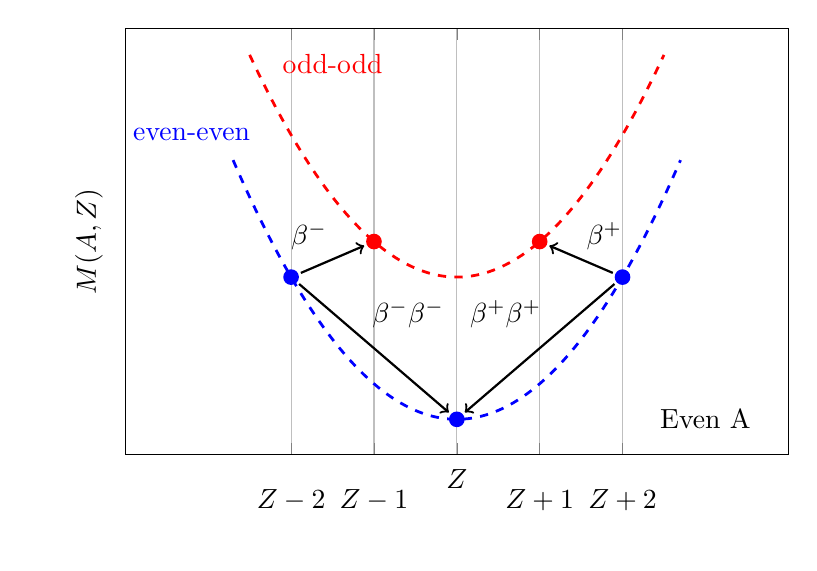
\begin{tikzpicture}
		\begin{axis}[
					grid,
					width=10cm, height = 7cm,
					xmin=-4, xmax=4,
					ymin=0, ymax=12,
					samples=100,
					ylabel={$M(A,Z)$},
					xtick={-2,-1,0,1,2},
					every axis y label/.style={at={(ticklabel cs: 0.5,-10)},rotate=90,anchor=south},
					xticklabels={$Z-2$,$Z-1$,$Z$,$Z+1$,$Z+2$},
					ytick=\empty,
					yticklabels={,},
					]
					% lower curve
			\addplot[mark=none,
					dashed, color=blue,
					line width=1pt,
					domain=-2.7:2.7
					] {x^2+1};
				\node (z-2)[fill=blue] at (axis cs:-2,5) {};
				\node (z)  [fill=blue] at (axis cs:0,1) {};
				\node (z+2)[fill=blue] at (axis cs:2,5) {};
			% upper curve
			\addplot[mark=none,
					dashed, color=red,
					line width=1pt,
					domain=-2.5:2.5
					] {x^2+5};
				\node (z-1)[fill=red] at (axis cs:-1,6) {};
				\node (z+1)[fill=red] at (axis cs:1,6) {};
			% arrows
			\draw [->, thick] (z-2) -- (z-1) node [midway,above left] {$\beta^-$};
			\draw [->, thick] (z-2) -- (z)   node [midway,auto] {$\beta^-\beta^-$};
			\draw [->, thick] (z+2) -- (z+1) node [midway,above right] {$\beta^+$};
			\draw [->, thick] (z+2) -- (z)   node [midway,above left] {$\beta^+\beta^+$};
			% text
			\node at (axis cs:-3.2,9) {\color{blue}even-even};
			\node at (axis cs:-1.5,11) {\color{red}odd-odd};
			\node at (axis cs:3,1) {Even A};
		\end{axis}
	\end{tikzpicture}
\end{document}
